% Main text of the article.  Derivations, checks and tables are in the Supplemental Material,
% ../theory/theory.tex (deterministic model) and ../demographic/demographic.tex (demographic noise).
% Build: latexmk -pdf paper.tex   (from this directory)
%
% Draft status (2026-10-11): restructured around the claim "life cycles explain the multiscaling
% shape; the self-limitation that makes them also caps sizes, so there is no Zipf law".  Numbers
% marked \todo{} come from scratch experiments and must be reproduced by a script in the repo
% before submission.
\documentclass[pre,twocolumn,superscriptaddress,nofootinbib]{revtex4-2}
\usepackage{amsmath,amssymb,bm}
\usepackage{graphicx}
\usepackage{xcolor}
\graphicspath{{../../assets/figures/}}
\usepackage[hidelinks]{hyperref}

\newcommand{\E}{\mathbb E}
\newcommand{\Var}{\operatorname{Var}}
\newcommand{\PhiN}{\Phi_{\mathcal N}}
\newcommand{\bPhi}{\bar\Phi}
\newcommand{\Sthr}{S_{\rm thr}}
\newcommand{\Sb}{\bar S}
\newcommand{\todo}[1]{\textcolor{red}{[TODO: #1]}}

\begin{document}

\title{Firm life cycles, multiscaling and the missing Zipf law in a scale-invariant
Lotka--Volterra economy}
\author{Ludovico Furlanetto}
\date{\today}

\begin{abstract}
We study a generalised Lotka--Volterra model of firms on a heterogeneous interaction network in
which interactions and self-limitation are measured in units of the mean firm size.  The economy
then grows at a rate selected by the dynamics, and in the large-$N$ limit the relative sizes obey the
standard disordered Lotka--Volterra equations with renormalised parameters.  Heterogeneous
dynamical mean-field theory gives the phase diagram on a power-law graph, with a closed form for
the stability line and a growth boundary that hardly depends on the network.  In the chaotic
phase each firm is a logistic unit driven by a Gaussian fitness whose mean and amplitude are set by
its degree.  For this one-firm problem a firm exits on the first fitness dip whose area exceeds
an explicit threshold, which gives its lifetime law.  Under the unbalanced panel used for firm
data a firm's volatility is its log range over its lifetime, so the size--volatility statistics are
those of firm life cycles.  Life cycles bend the multiscaling ratio curve below the
fixed-shape line, as in Compustat, and give a cross-sectional spread of volatilities with a
power-law tail close to the empirical one.  With demographic noise in place of the immigration floor,
the size--volatility relation becomes a crossover from slope $-1/2$ to $0$ with an effective exponent
$0.16$--$0.20$ over two decades.  The model does not produce a Zipf law.  We show why: the
self-limitation that generates the life cycles and the volatility decline also caps firm size,
so the size range over which volatility falls and the volatility exponent trade off against each
other, and giving each firm its own scale removes the size dependence altogether.
\end{abstract}

\maketitle

%----------------------------------------------------------------------
\section{Introduction}

Large firms grow less erratically than small ones, but not by as much as independent subunits
would imply.  If $v_i$ is the volatility of firm $i$'s growth rate and $\Sb_i$ its mean size, the
conditional moments in Compustat scale as $\E[v^q\mid\Sb]\sim\Sb^{-\zeta_q}$ over four decades of size,
with $\beta=\zeta_1\approx0.2$ \cite{stanley1996,amaral1997,sutton2002,moran2024}.  The ratio curve
$\zeta_q/\zeta_1\approx2.0$, $2.6$, $2.9$ for $q=2,3,4$ bends below the line $\zeta_q/\zeta_1=q$ of a
volatility law of fixed shape; the volatility rescaled by its size-conditional mean has a
universal distribution with a power-law tail of exponent $-(1+b)$, $b\simeq4.6$; and the rescaled growth
rates stay fat-tailed at every size, with no sign of the Gaussianisation that sums of independent
units would produce \cite{moran2024}.  Firm sizes themselves follow Zipf's law \cite{axtell2001}.
Granular models, in which a firm is a sum of subunits, account for the slow decline but not for
the universality and the absence of Gaussianisation \cite{wyartbouchaud2003,moran2024}, and data
that include small firms show a steep decline for small firms and a nearly flat one for large firms
rather than a single power law \cite{fontanelli2025}.

Disordered Lotka--Volterra (GLV) communities with weak immigration have a chaotic phase in which
species keep exchanging the roles of rare and dominant \cite{roy2020,mallmin2024}.  Each species then
behaves as a logistic unit driven by a coloured Gaussian field \cite{mallmin2024}, and in the limit
of vanishing immigration its trajectory is a jump process: long stretches of rarity, a sudden bloom
and a gradual decline \cite{arnouxbunin2024}.  This literature uses fully connected interactions and a
fixed carrying capacity, and reads off ecological observables.  Here we ask what the same
dynamics implies for firms.

We use the GLV with interactions and self-limitation measured in units of the mean firm size,
on a scale-free interaction network.  The model is scale invariant: the economy grows at a rate the
dynamics selects.  For relative sizes this is a reformulation rather than a new dynamical system,
since at large $N$ it maps onto the standard GLV with renormalised parameters (Sec.~\ref{sec:model});
the new ingredients are the heterogeneous network, the growth rate as an output, and the firm-growth
observables.  Our results are of three kinds.  (i) The phase diagram of the chaotic phase on a
power-law graph from heterogeneous dynamical mean-field theory (HDMFT), and the degree-resolved law
of the field each firm feels (Secs.~\ref{sec:phase} and~\ref{sec:onefirm}).  (ii) A theory of firm
life cycles: an exact solution of the one-firm equation, a rule that predicts which fitness dip ends
a firm, its lifetime law, and a criterion that ties the multiscaling of the size--volatility
relation to the spread of lifetimes (Sec.~\ref{sec:life}); demographic noise turns the result into a
crossover law (Sec.~\ref{sec:demog}).  (iii) A comparison with the firm-growth facts that is explicit
about what the mechanism does not explain (Sec.~\ref{sec:data}), and an argument that it cannot
produce a Zipf law together with a volatility law spanning many decades (Sec.~\ref{sec:zipf}).
Derivations, checks and further results are in the Supplemental Material (SM).

%----------------------------------------------------------------------
\section{Model}
\label{sec:model}

Firm $i=1,\dots,N$ has size $x_i$, and $m=N^{-1}\sum_jx_j$ is the mean size.  The relative GLV is
\begin{equation}
  \dot x_i=x_i\Bigl[1-\frac{x_i}{m}+\frac1m\sum_jW_{ij}x_j\Bigr]+\lambda(m-x_i),
  \label{eq:model}
\end{equation}
with $W_{ij}=A_{ij}(\mu/C+\sigma z_{ij}/\sqrt C)$ on a configuration-model graph of degree law
$p(k)\propto k^{-\alpha}$ and mean degree $C$, independent Gaussian $z_{ij}$ (no reciprocity), and $\mu<0$
for competition.  Every term is homogeneous of degree one in $x$, so the economy has no preferred
size.  The immigration term $\lambda(m-x_i)$ is an influx of small firms at rate $\lambda m$ plus a uniform
exit at rate $\lambda$; it keeps firms above a floor and sums to zero.  We use $N=8000$, $C=N/40$,
$\lambda=10^{-3}$, $\alpha\in[2.2,6]$, and the operating point $(\mu,\sigma)=(-1.76,1.75)$.

With relative sizes $S_i=x_i/m$,
\begin{equation}
  \frac{\dot m}{m}=g(t)=\langle SF\rangle,\qquad
  \dot S_i=S_i\bigl[F_i-g(t)\bigr]+\lambda(1-S_i),
  \label{eq:replicator}
\end{equation}
with $F_i=1-S_i+(WS)_i$: the scale grows at the share-weighted mean fitness, and the composition is
a replicator equation.  Writing $\Phi_i=1-g+(WS)_i$ for the \emph{fitness} of firm $i$,
\begin{equation}
  \frac{d\ln S_i}{dt}=\Phi_i(t)-S_i+\lambda\bigl(S_i^{-1}-1\bigr),
  \label{eq:firm}
\end{equation}
a logistic equation with a moving carrying capacity.  Averaging over any stationary stretch gives
$\Sb_i=\bPhi_i$ up to the floor term: a firm's mean size is its mean fitness.

\paragraph{Relation to the standard GLV.}
If the growth rate self-averages to a constant $g^*$ at large $N$, the substitution $S=r\,y$,
$t'=r\,t$ with $r=1-\lambda-g^*$ turns Eq.~\eqref{eq:replicator} into
$dy_i/dt'=y_i[1-y_i+(Wy)_i]+\lambda/r^2$, the migration-supported GLV of
Refs.~\cite{bunin2017,mallmin2024,arnouxbunin2024} on the same graph.  The stationary statistics of
relative sizes are therefore those of the standard model with renormalised immigration, and on a
fully connected graph they are the ones studied in Refs.~\cite{mallmin2024,arnouxbunin2024}.  What the
normalisation adds is the growth rate $g^*$ as an output, fixed by $\langle S\rangle=1$, which gives the
growth boundary of Sec.~\ref{sec:phase}; a common mode $g(t)-g^*$ at finite $N$; and observables
defined, as in firm data, relative to the mean firm.  It also fixes the scale of the demographic
noise of Sec.~\ref{sec:demog}, which in the absolute model would set a size.

%----------------------------------------------------------------------
\section{Mean-field theory and phase diagram}
\label{sec:phase}

For $C\to\infty$ the field on a firm of relative degree $\kappa=k/C$ becomes Gaussian.  The HDMFT
replaces Eq.~\eqref{eq:firm} by one stochastic process per degree class, closed by
self-consistent averages over neighbours, which are drawn in proportion to degree
\cite{aguirrelopez,patil2026}.  For an uncorrelated kernel the fitness is
\begin{equation}
  \Phi(t)=1-g(t)+\mu\kappa\bar B+\sigma\sqrt\kappa\,\xi(t),
  \label{eq:fitness}
\end{equation}
with $\E[\xi(t)\xi(t')]=Q(t-t')$, and $\bar B$ and $Q$ degree-weighted averages of $S$ and
$S(t)S(t')$.  The structural cutoff of the hubs is handled with a soft-configuration kernel
\cite{patil2026}.  Previous network analyses of the GLV treat the fixed points
\cite{aguirrelopez,patil2026}; here we need the boundary of the chaotic phase.

\paragraph{Stability line.}
If the composition relaxes, the stationary abundances are clipped Gaussians and the unique fixed
point loses stability when the Perron root of $\sigma^2\varphi_pK_{pr}$ reaches one, with $\varphi_p$
the survival fraction of class $p$ and $K_{pr}$ the connection kernel.  On a regular graph the
mean interaction is a uniform shift that cancels in the replicator, and
$\sigma_c=\sqrt2/(1+\gamma)$ for coupling reciprocity $\gamma$, independent of $\mu$.  On a
heterogeneous, uncorrelated graph the stability operator has rank one, and the threshold reduces
to two scalar equations: with $\Delta_\kappa=A\kappa^{-1/2}+M\kappa^{1/2}$ and $w_n(\Delta)=\int_{-\Delta}^\infty
(\Delta+z)^n\,\phi(z)\,dz$,
\begin{equation}
  \begin{gathered}
  \sigma_c^{-2}=\bigl\langle\kappa^2\PhiN(\Delta_\kappa)\bigr\rangle,\\
  \bigl\langle\kappa^2\Delta_\kappa w_1(\Delta_\kappa)\bigr\rangle=0,\qquad
  M=\mu\bigl\langle\kappa^{3/2}w_1(\Delta_\kappa)\bigr\rangle .
  \end{gathered}
  \label{eq:sigmac}
\end{equation}
To first order in the degree variance,
\begin{equation}
  \sigma_c(\mu)\simeq\sqrt2\Bigl[1-\frac{\Var\kappa}{2}\Bigl(1-\frac{\mu^2}{2\pi}\Bigr)\Bigr].
  \label{eq:sigmac-v}
\end{equation}
Degree heterogeneity lowers the threshold, because hubs feel noise of amplitude $\propto\sqrt\kappa$.
A mean interaction of either sign raises it; beyond first order competition raises it more,
because it removes the noisiest firms.  Equation~\eqref{eq:sigmac} agrees with the full HDMFT to
$0.002$ at $\alpha=6$ and $0.03$ at $\alpha=3.5$ (SM).  Heavy-tailed graphs are the least stable at weak
competition and the most stable at strong competition (Fig.~\ref{fig:phase}b).

\paragraph{Growth.}
Since $g^*=1-a$ for the fixed-point closure, the zero-growth line follows by fixing $a=1$.  On a
regular graph it is $\mu^{(0)}=-g_0(\sigma)$, with $g_0=1-\Delta/w_1(\Delta)$ and $\sigma^2w_2(\Delta)=1$.
Heterogeneity shifts it by $c(\sigma)\Var\kappa$, with $c$ running from $0$ at weak disorder to
$5/4-\pi/2\simeq-0.32$ at $\sigma_c$.  The coefficient is at most a third of that of $\sigma_c$, which is
why the growth boundary hardly depends on the topology.  Its continuation above $\sigma_c$ tracks the
simulated contour to $0.03$ in $\mu$ (Fig.~\ref{fig:phase}a).

\begin{figure*}[t]
  \centering
  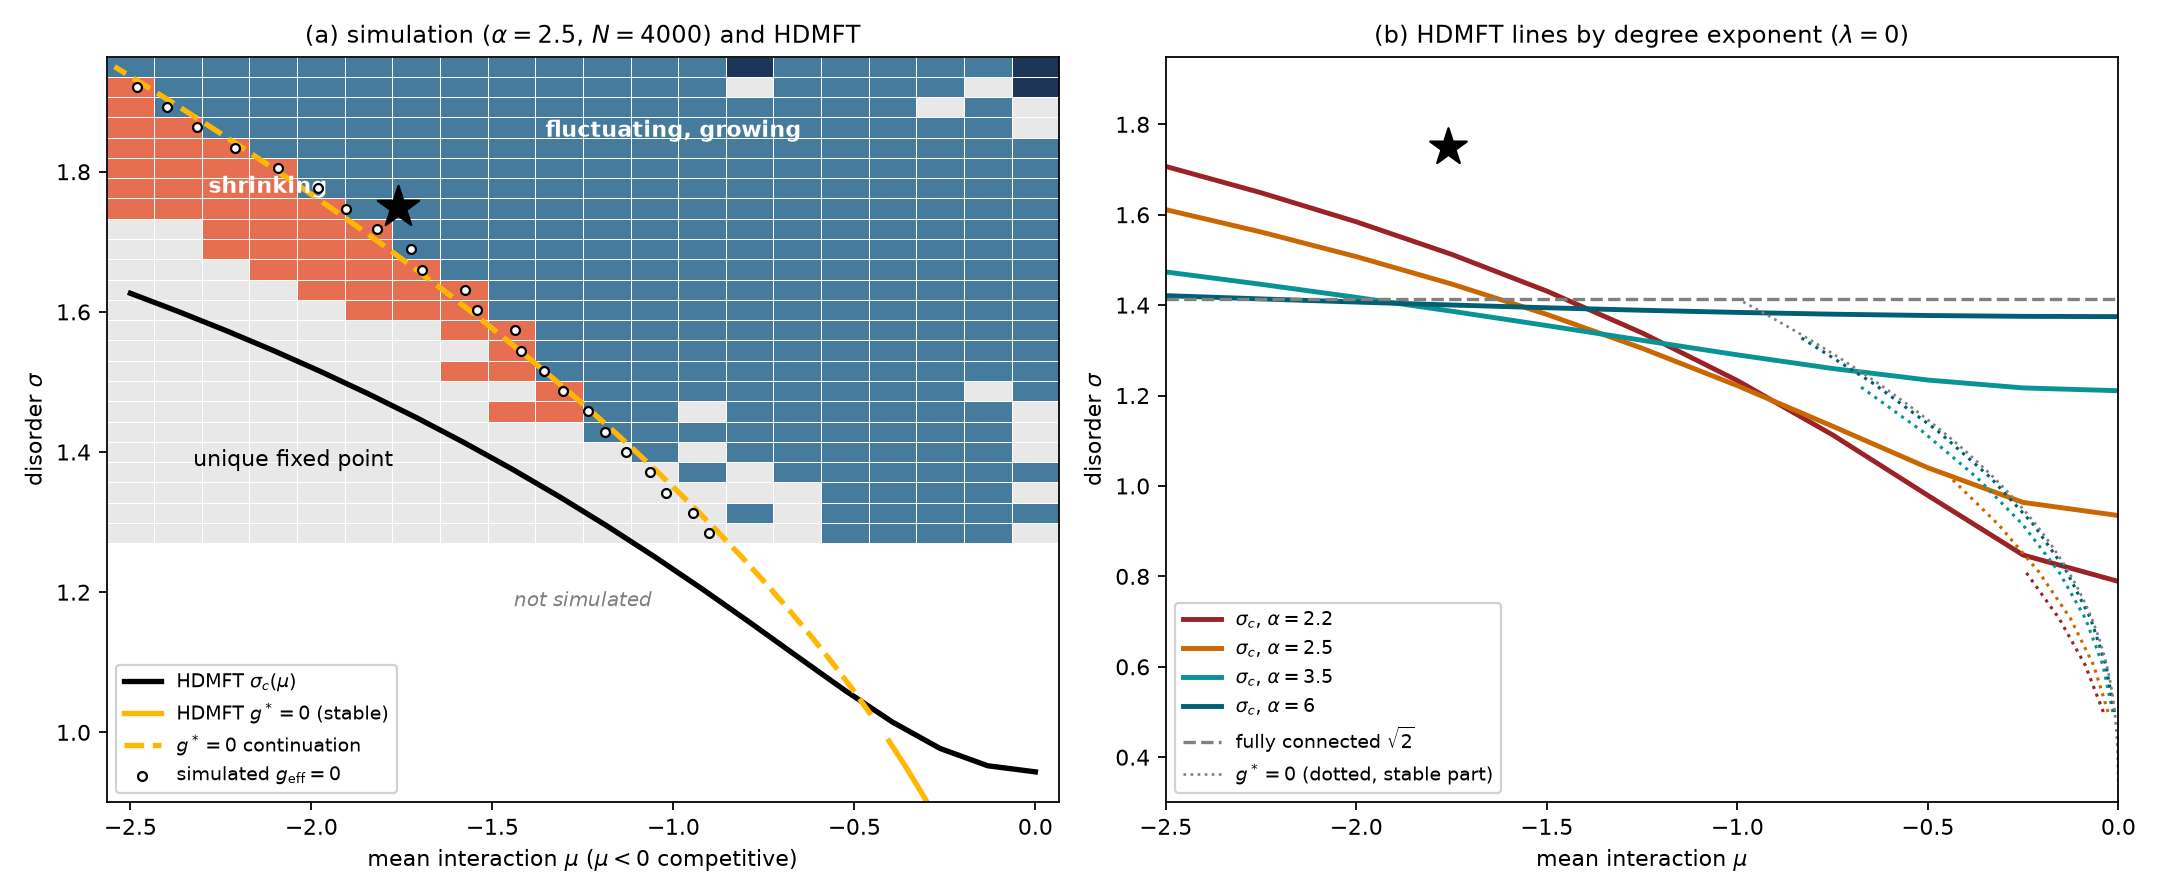
\includegraphics[width=\textwidth]{phase_theory.png}
  \caption{(a) Phase diagram for $\alpha=2.5$ ($N=4000$, $C=100$, $\lambda=10^{-3}$).  Regions
  from the HDMFT: below the stability line $\sigma_c(\mu)$ (black; 60 classes, SCM kernel) the
  composition has a unique fixed point; above it chaos coexists with trapping equilibria.  The
  zero-growth line (white; dashed where it continues an unstable fixed point) separates growing from
  shrinking economies.  Symbols are simulation: zero crossings of the growth rate, the $\sigma$ above
  which the median churn exceeds $0.035$ (hollow where it is already exceeded at the lowest simulated
  $\sigma=1.28$), cells whose integration failed, and the operating point.
  (b) Stability line for $\alpha=2.2$--$6$ ($\lambda=0$) with the closed form for the bilinear kernel
  (dashed, where that kernel is a probability) and the regular-graph value $\sqrt2$.  (c) Fraction of
  runs chaotic at $T=1600$ against the distance from each graph's own $\sigma_c$, ten graphs per point.}
  \label{fig:phase}
\end{figure*}

\paragraph{Above the line.}
Below $\sigma_c$ three different initial conditions freeze into the same state.  At $\sigma_c$ no
simulated run is chaotic.  Above it, runs are either trapped in one of many stable equilibria or
chaotic with a persistent amplitude, and which one depends on the realisation: at $\mu=-1.97$ the
chaotic fraction of ten graphs is $0.2$, $0.1$, $0.8$ and $1$ at $\sigma-\sigma_c=0.025$, $0.05$, $0.1$
and $0.2$, and at $\mu=-1.05$ chaos takes over only by $\sigma_c+0.2$ (Fig.~\ref{fig:phase}c).  This is the
multiple-attractor regime of the disordered GLV.  A simulated ``freezing line'' that classifies
cells by the churn of their growth rates lies $0.1$--$0.3$ above $\sigma_c$ and is a statistic of this
coexistence region, not a second transition.  The region of failed integrations at weak
competition and strong disorder is a numerical artefact of the solver tolerance: there the
economy is strongly concentrated and grows fast, but stays bounded.

%----------------------------------------------------------------------
\section{Firms as independent units}
\label{sec:onefirm}

At the operating point the composition never settles: over a few hundred time units most firms
fall to the floor and climb back.  As in the fully connected case \cite{mallmin2024}, a firm can be
replaced by a logistic unit in a Gaussian field; on the network the field's law depends on the
degree.  Within a firm, $\Phi_i=\bPhi_i+f_i\eta_i(t)$ with $\eta_i$ a smooth unit-variance process of
correlation time $\tau$, and at fixed degree Eq.~\eqref{eq:fitness} gives
\begin{equation}
  \bPhi\mid\kappa\sim\mathcal N\bigl(r_\kappa,\;\sigma^2\kappa Q_T\bigr),\qquad
  f_\kappa=\sigma\sqrt{\kappa(Q_0-Q_T)},
  \label{eq:law}
\end{equation}
with $r_\kappa=1-\bar g+\mu\kappa\bar B$ and $Q_T$ the part of $Q$ that is static over a window.
Five numbers and the degree law fix the fitness of every firm.  Measured firm by firm in the full
model, the static field is Gaussian once its predicted mean and spread are removed, the amplitude
grows as $\sqrt\kappa$ over the whole degree range, and the strong skew of $\bPhi$ on heavy-tailed
graphs comes from the mixture over degrees (Fig.~\ref{fig:fitness}).

\begin{figure*}[t]
  \centering
  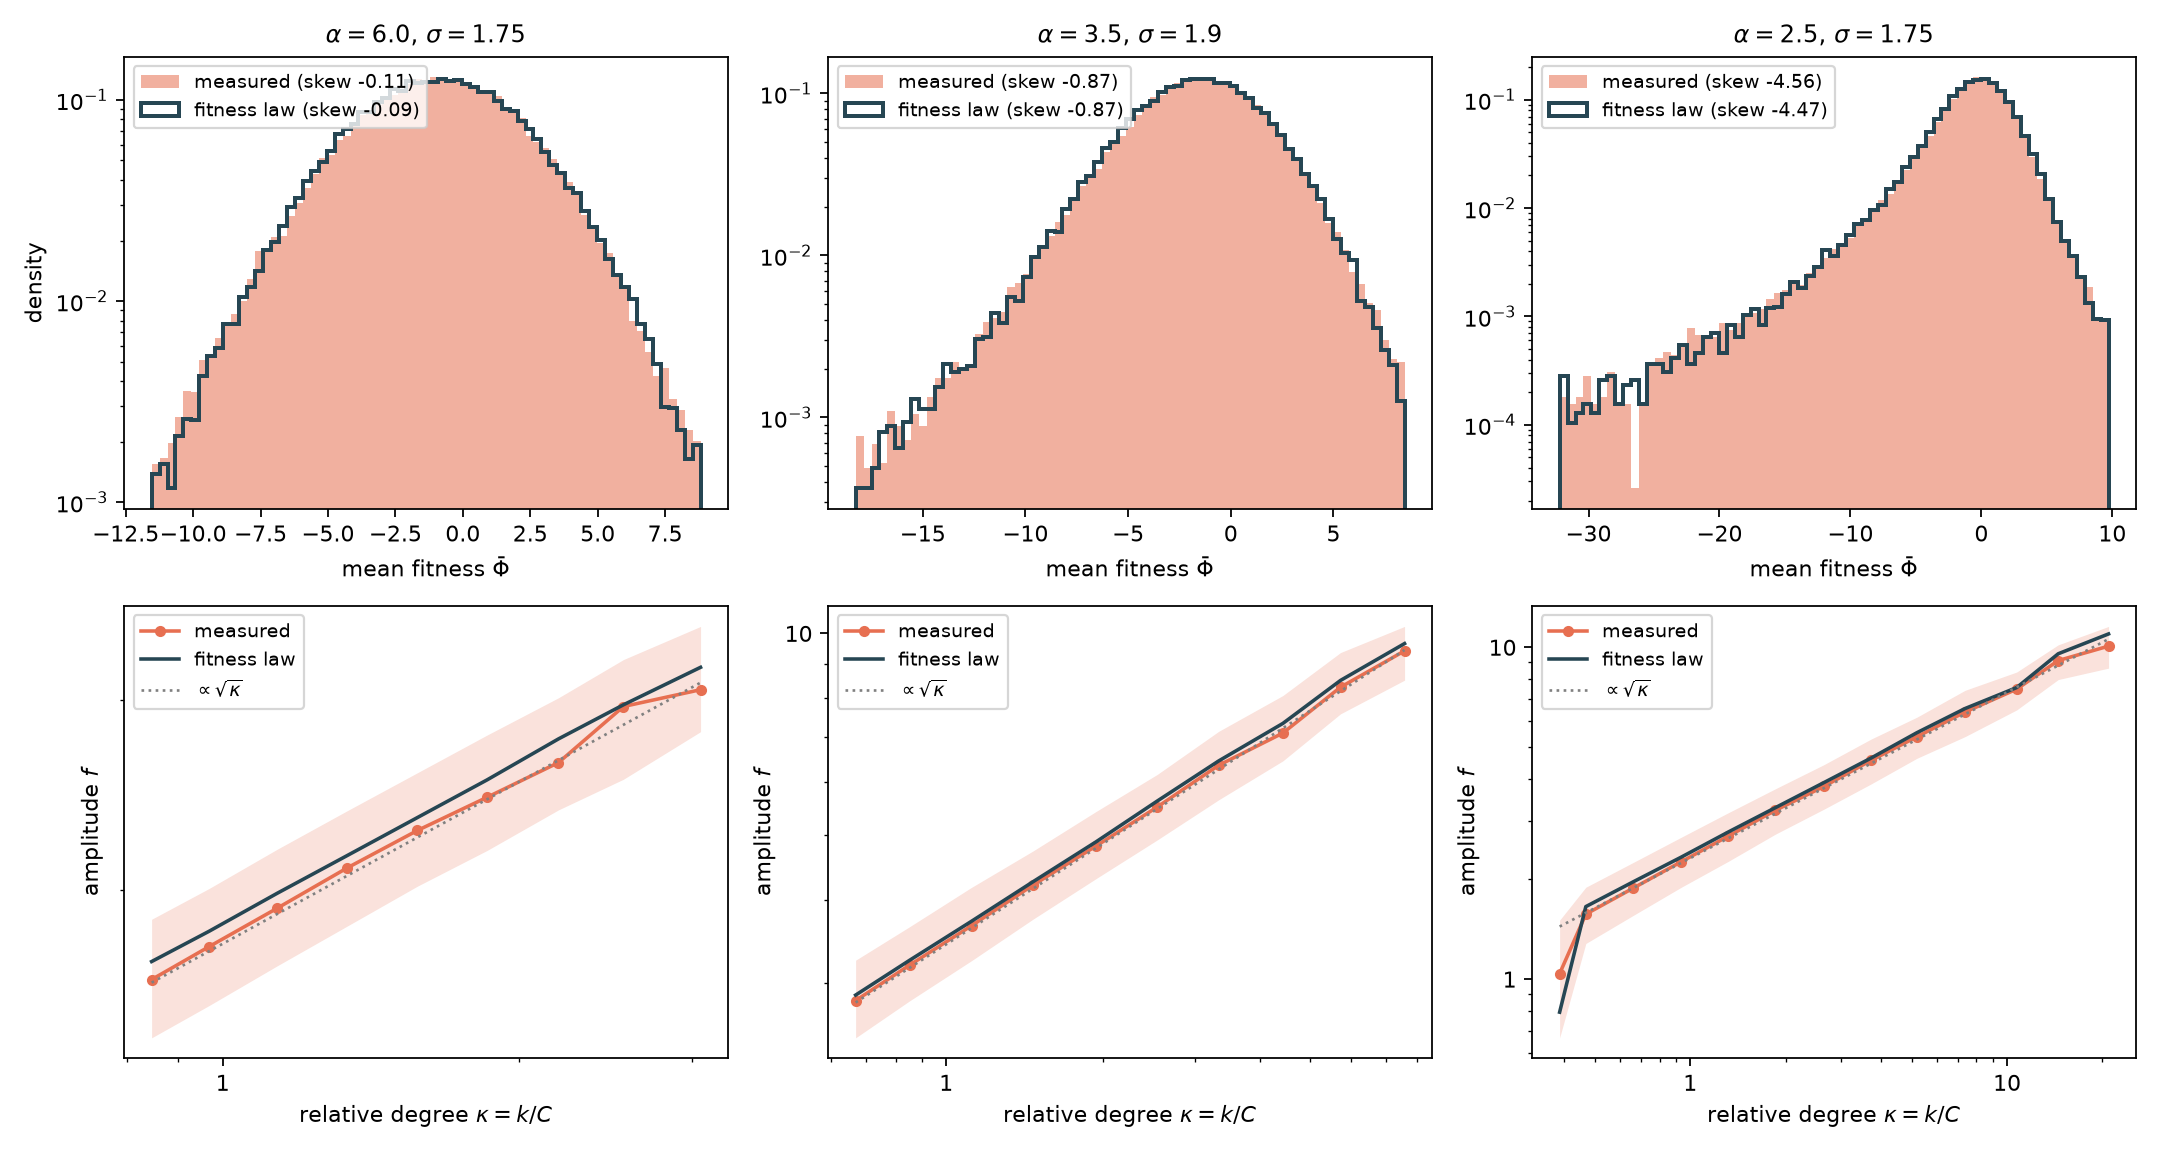
\includegraphics[width=0.9\textwidth]{fitness_law.png}
  \caption{The fitness law against the full model.  Top: per-firm mean fitness, measured and sampled
  from Eq.~\eqref{eq:law}.  Bottom: fitness amplitude against relative degree (median and quartiles),
  with $f\propto\sqrt\kappa$.}
  \label{fig:fitness}
\end{figure*}

Replacing the network by independent copies of Eq.~\eqref{eq:firm}, each driven by a Gaussian
fitness with its firm's measured $(\bPhi_i,f_i)$, reproduces the size--volatility exponent of the
full model to $0.02$ on every graph and its ratio curve to $0.25$ (SM).  The size--volatility
statistics are therefore properties of a single firm and of the distribution of fitness across
firms; the network enters only through Eq.~\eqref{eq:law}.

%----------------------------------------------------------------------
\section{Life cycles}
\label{sec:life}

Firm data form an unbalanced panel: every firm contributes over its own listed life
\cite{moran2024}.  In the model a firm is listed while $S>\Sthr$, and each listed spell counts as one
firm.  Its volatility is the MAD estimate $v=\sqrt{\pi/2}\,\overline{|g_t-\bar g|}$ of its growth rates
$g_t=\Delta\ln S$ over $n$ steps.  For a spell that enters and leaves at $\Sthr$, exactly,
\begin{equation}
  v=\sqrt{\tfrac\pi2}\;\frac{2\ell+V_p}{n},\qquad\ell=\ln\frac{S_{\max}}{\Sthr},
  \label{eq:identity}
\end{equation}
with $V_p\ge0$ the variation in excess of one rise and fall.  Spells shorter than about $8\tau$ have
$V_p\simeq0$: a spell is a single hump in $\ln S$, and longer spells are a few humps merged by
fitness dips that did not end them.  A firm's volatility is thus essentially its log range over
its lifetime.

\paragraph{Exact solution and kill rule.}
At $\lambda=0$ Eq.~\eqref{eq:firm} is linear in $1/S$.  With $\mathcal A(t)=\int^t\Phi$,
\begin{equation}
  \frac1{S(t)}=\int_{-\infty}^te^{-[\mathcal A(t)-\mathcal A(t')]}\,dt' ,
  \label{eq:exact}
\end{equation}
so the size is a soft minimum over drawdowns of the integrated fitness.  Near a downcrossing of
$\Phi$ with slope $-s$ the solution is an inverse Mills ratio, and during a dip
$S\simeq\sqrt{s/2\pi}\,e^{-[\mathcal A(t_0)-\mathcal A(t)]}$.  A spell therefore ends at the first
negative excursion of the fitness whose area exceeds
\begin{equation}
  \ell_c(s)=\ln\frac{\sqrt{s/2\pi}}{\Sthr},
  \label{eq:kill}
\end{equation}
with no fitted constant; the rule classifies $96$--$98\%$ of dips correctly (Fig.~\ref{fig:life}a).
This is the finite-floor counterpart of the jump-process picture of Ref.~\cite{arnouxbunin2024}:
the bloom is the climb from the floor, and the kill rule decides which decline ends the life.

\paragraph{Lifetime law.}
Dips occur at Rice's rate $\nu(u)=e^{-u^2/2}/2\pi\tau$, with $u=\bPhi/f$, and end the spell with
probability $P_{\rm kill}(u)$, a level-crossing statistic of the Gaussian fitness computable from
the Slepian model.  The mean lifetime is
\begin{equation}
  \bar L(u)=\frac{\PhiN(u)}{\nu(u)\,P_{\rm kill}(u)},
  \label{eq:lifetime}
\end{equation}
which matches the one-firm process to $3\%$ for $u\ge1$ with no simulation input
(Fig.~\ref{fig:life}b,c).  For $u\gg1$ dips are short parabolae and
$-\ln P_{\rm kill}\simeq\tfrac12(3\ell_c/2f\tau)^{2/3}u^{4/3}$, so lifetime grows faster than any power of
size: the size--volatility exponent of the life-cycle part is an effective exponent that increases
along the size range.

\begin{figure*}[t]
  \centering
  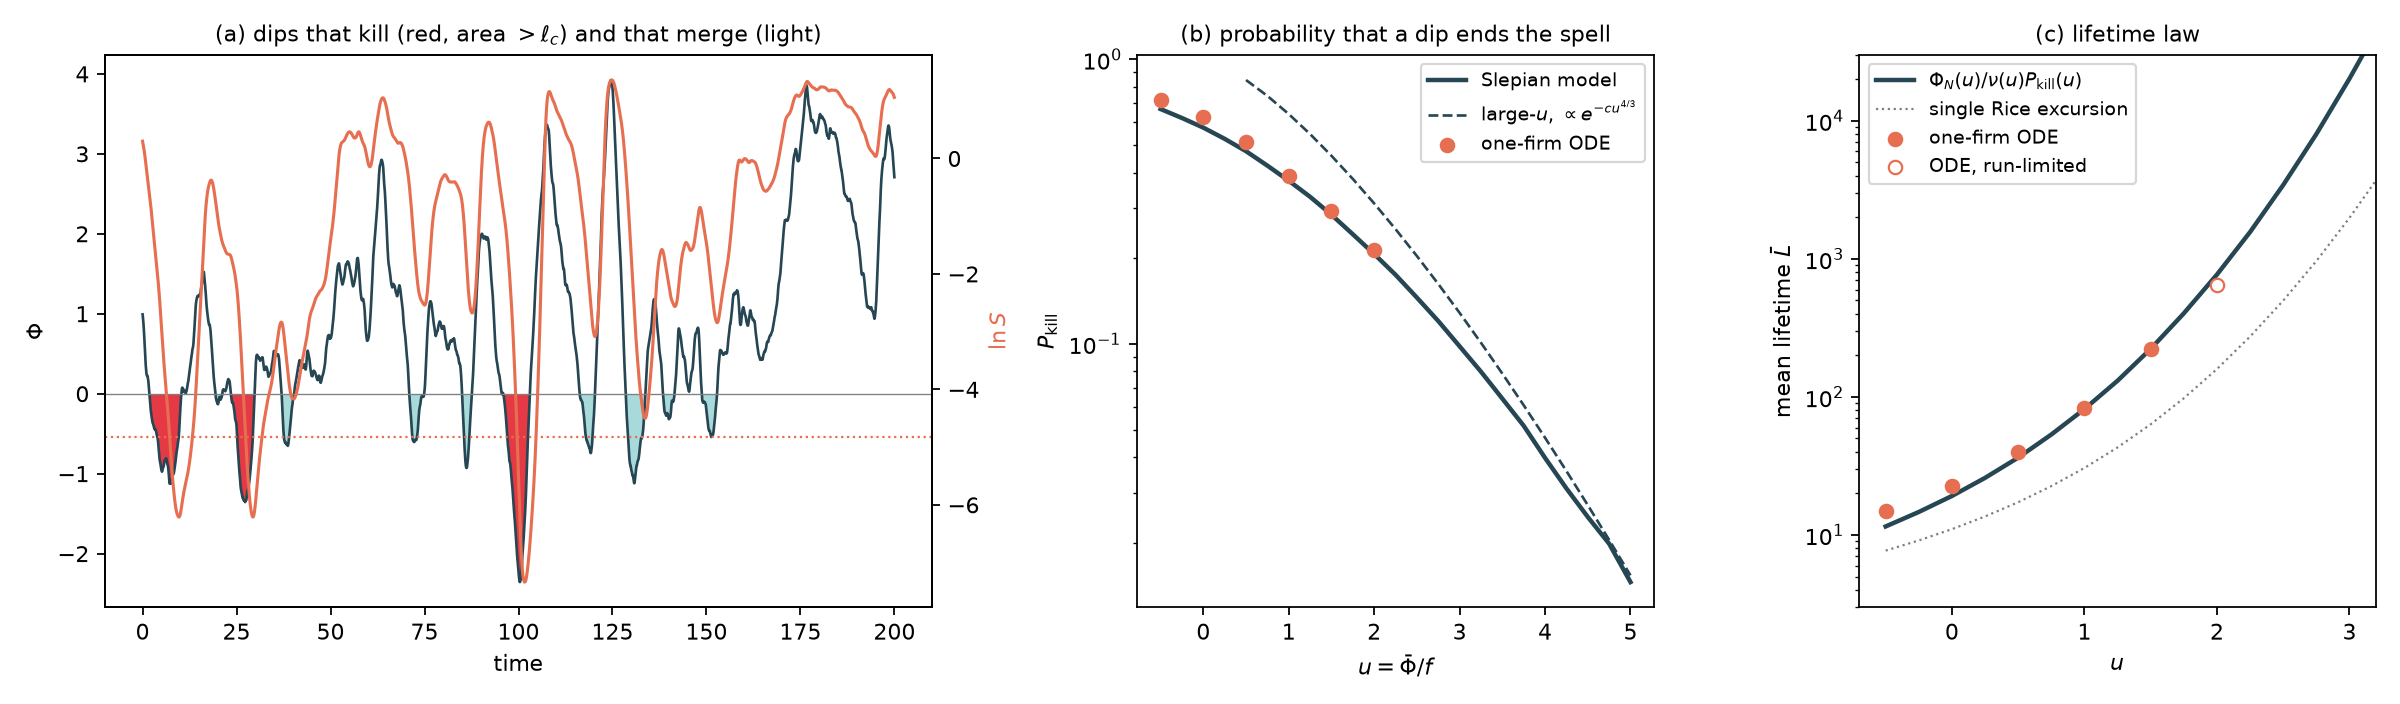
\includegraphics[width=\textwidth]{lifetime_law.png}
  \caption{Kill rule and lifetime law ($\alpha=6$ fitness).  (a) A fitness path: dips with area above
  $\ell_c(s)$ (red) end the spell, as $\ln S$ (right axis) crosses the threshold (dotted); light dips
  merge excursions.  (b) $P_{\rm kill}$: one-firm process, Slepian model and large-$u$ asymptote.
  (c) Mean lifetime: one-firm process against Eq.~\eqref{eq:lifetime}; the hollow point is biased by the
  run length.}
  \label{fig:life}
\end{figure*}

\paragraph{Multiscaling.}
Write $v=A(\Sb)X$ with $X$ random at fixed size.  If $c_n$ are the cumulants of $\ln X$ at fixed
$\Sb$, then exactly
\begin{equation}
  \zeta_q-q\,\zeta_1=-\sum_{n\ge2}\frac{q^n-q}{n!}\,\frac{dc_n}{d\ln\Sb},
  \label{eq:criterion}
\end{equation}
so a volatility law of fixed shape, $X$ independent of $\Sb$, gives $\zeta_q=q\zeta_1$ exactly, and at
second-cumulant order the ratio curve bends below $q$ if and only if $\Var(\ln X\mid\Sb)$ grows with
size.  The bend of the data therefore requires a source of volatility dispersion that grows with
size.  For life cycles $X=\ell/n$ and the spread is that of $\ln n$.  Small firms live through a
single fitness excursion, of fairly regular length; large firms exit on rare, memoryless kills, for
which $\Var\ln n=\pi^2/6$.  In the one-firm process $\Var(\ln n\mid\Sb)$ rises from $0.29$ to $0.65$
across the larger half of spells, and $\Var\ln L$ reaches $\pi^2/6$ at $u\simeq1.5$.  The bend is
therefore a crossover between two kinds of exit.  On heavy-tailed graphs the spread of fitness
amplitudes, $f\propto\sqrt\kappa$, adds lifetime dispersion at fixed size and flattens the ratio curve
further; making $f$ homogeneous restores the plain life-cycle bend (SM).

%----------------------------------------------------------------------
\section{Demographic noise}
\label{sec:demog}

The floor $\lambda$ is a modelling device, and it produces the calm, brief spells near the listing
threshold that make the size--volatility curve humped at small sizes (Sec.~\ref{sec:data}).  We
replace it by the birth--death noise of stochastic Lotka--Volterra models \cite{altieri2021},
\begin{equation}
  dx_i=x_i\Bigl[1-\frac{x_i}{m}+\frac1m\sum_jW_{ij}x_j\Bigr]dt+\sqrt{D\,m\,x_i}\;dW_i ,
  \label{eq:demog}
\end{equation}
with exit at $x_i=0$ and a newborn of size $Dm$ taking the node.  The noise unit $Dm$ scales with the
economy, so the model stays scale invariant and $D$ replaces $\lambda$ without adding a parameter.
The one-firm reduction still holds: driving each node with its measured field and fresh noise
reproduces the full life panel to $0.01$ in $\beta$, $0.05$ in the ratios and $2\%$ in exit rates
(SM).

\paragraph{Phase line.}
With turnover each node is a renewal process whose stationary law is exact, $p(x\mid h)=s(\min(x,D))\,
m(x)/T(D)$ in terms of the scale and speed densities of the one-firm diffusion at field $h$.  A
static cavity theory built on it gives the instability line $\sigma_c(D)$, which tends to the
deterministic line as $D\to0$ ($1.399$ against $1.400$ at $\alpha=6$) and rises almost linearly with the
noise, from $1.460$ to $1.577$ at $\alpha=2.5$ between $D=0.003$ and $0.3$.  It predicts the turnover
rate to $0.5\%$ below $\sigma_c$ and $1.5\%$ above it (SM).

\paragraph{Volatility law.}
Splitting $\ln S$ into the noise-free response to the field and a linear fluctuation that relaxes
at the local rate $S$ gives, for a firm's growth over a step $\Delta t$,
\begin{equation}
  \Var g\simeq V_F+\Bigl\langle\frac{D}{S^2}\bigl(1-e^{-S\Delta t}\bigr)\Bigr\rangle_{\rm life},
  \label{eq:vlaw}
\end{equation}
which matches the measured volatility to within $5\%$ over a decade and a half of $\Sb$ (SM).  The
fitness part $\sqrt{V_F}\simeq0.25$--$0.32$ is nearly independent of size, the demographic part falls as
the inverse square root of size and faster for large firms.  The size--volatility relation is
therefore a crossover from slope $-1/2$ to slope $0$, the shape reported for French firms
\cite{fontanelli2025}.  At $\alpha=2.5$, $\sigma=1.75$, $D=0.1$ ($N=32000$) the two regimes blend into a nearly
straight decline: for lives of at least $10$ steps $\beta=0.16$ with ratios $1.76$, $2.28$, $2.58$ over
$1.8$ decades, and for at least $20$ steps $\beta=0.20$ with ratios $1.77$, $2.33$, $2.71$, the curve
flattening slightly at the top as in the data (Fig.~\ref{fig:demog}).

\begin{figure*}[t]
  \centering
  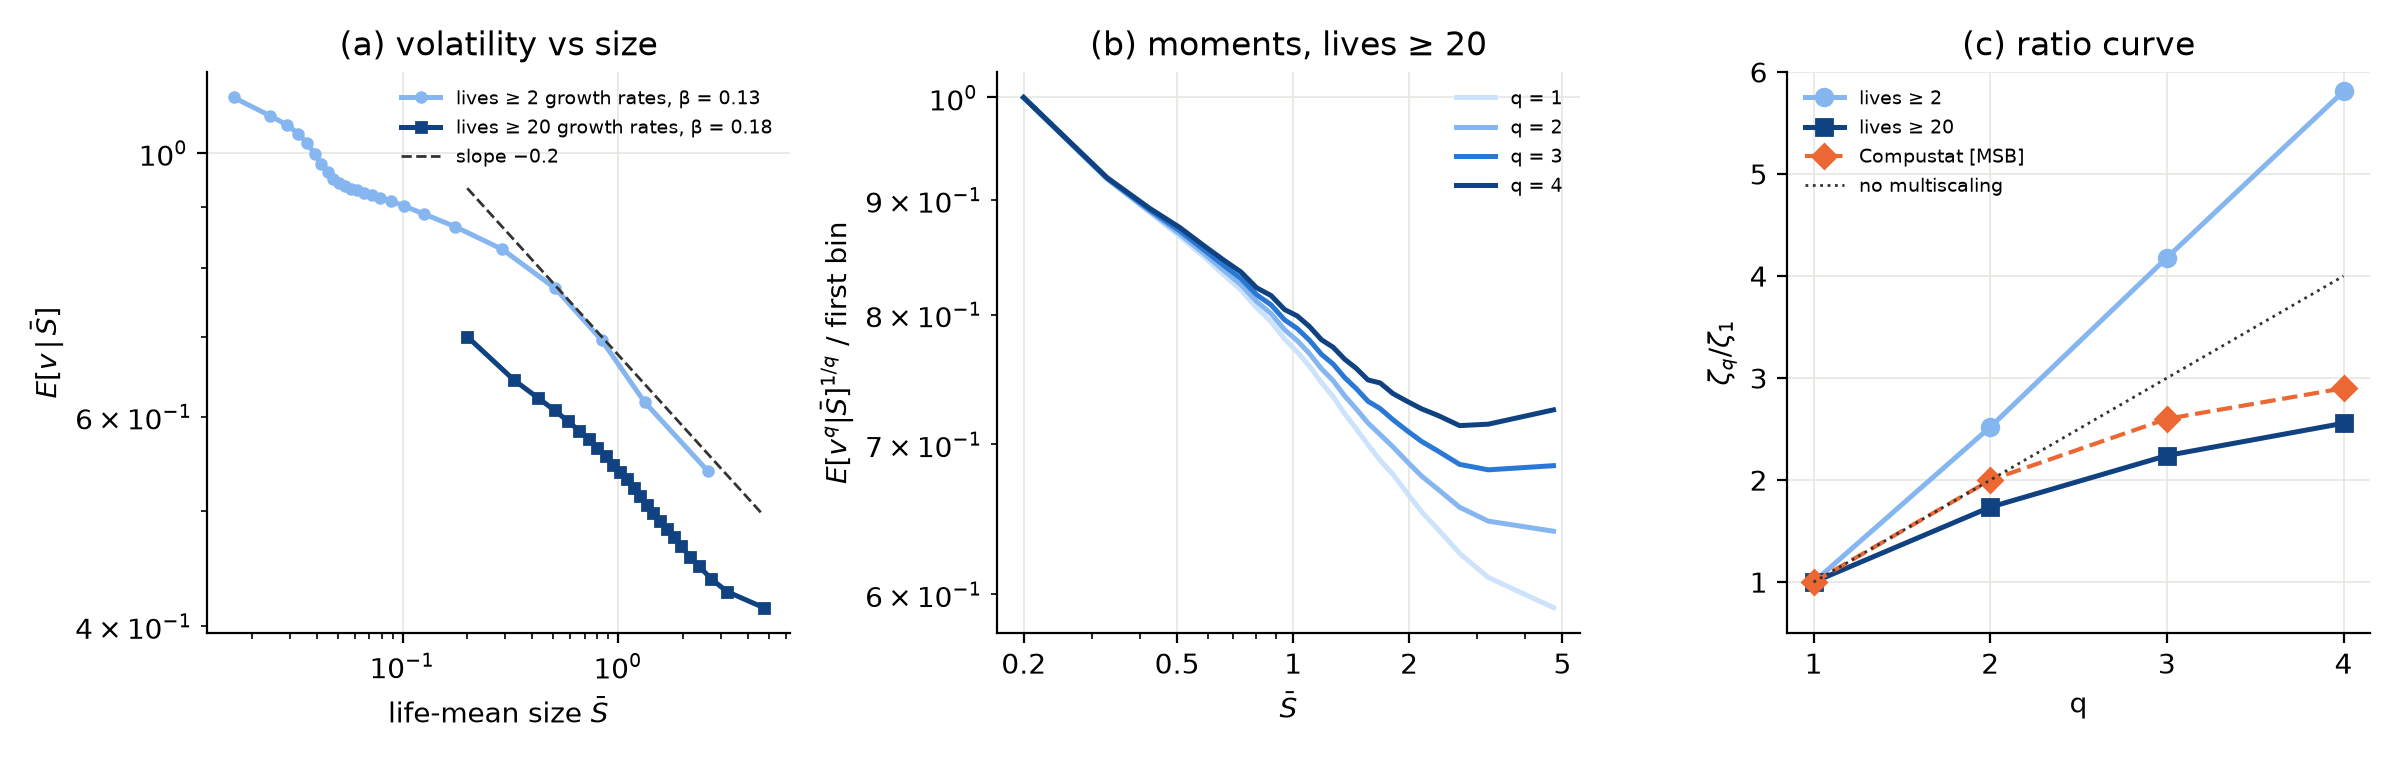
\includegraphics[width=\textwidth]{demographic_life_panel.png}
  \caption{Life panel with demographic noise ($\alpha=2.5$, $\sigma=1.75$, $D=0.1$, $N=32000$, $C=200$,
  eight economies pooled).  (a) Mean volatility against life-mean size.  (b) Moments $q=1$--$4$ for
  lives of at least $20$ steps.  (c) Ratio curves against Compustat \cite{moran2024}.}
  \label{fig:demog}
\end{figure*}

%----------------------------------------------------------------------
\section{Comparison with data}
\label{sec:data}

Table~\ref{tab:data} collects the size--volatility statistics.  For the deterministic model the
binned volatility has a hump at small sizes, made of spells that barely clear the listing threshold,
and a flat top that makes a peak-started fit unstable, so we fit on the larger half of spells by
size, which fixes $\beta$ to $\pm0.03$ between realisations.  The demographic rows use all $25$ bins.

\begin{table}[b]
\caption{Size--volatility statistics.  Deterministic model: spell panel, larger half of spells,
medians over eight economies.  Demographic noise: life panel, all bins, $N=32000$.}
\label{tab:data}
\begin{ruledtabular}
\begin{tabular}{lcc}
 & $\beta$ & $\zeta_q/\zeta_1$, $q=2,3,4$\\
\hline
$\alpha=6$, $\sigma=1.75$ & $0.55$ & $1.84$, $2.50$, $3.00$\\
$\alpha=3.5$, $\sigma=1.9$ & $0.28$ & $1.79$, $2.30$, $2.53$\\
$\alpha=2.5$, $\sigma=1.75$ & $0.19$ & $1.42$, $1.34$, $0.95$\\
noise, $D=0.1$, $n\ge10$ & $0.16$ & $1.76$, $2.28$, $2.58$\\
noise, $D=0.1$, $n\ge20$ & $0.20$ & $1.77$, $2.33$, $2.71$\\
Compustat \cite{moran2024} & $0.15$--$0.20$ & $2.0$, $2.6$, $2.9$\\
\end{tabular}
\end{ruledtabular}
\end{table}

\paragraph{What the mechanism explains.}
The shape of the multiscaling is robust: the ratio curve bends below $q$ by about the empirical
amount on weakly heterogeneous graphs and with demographic noise, and it does not depend on the fit
range.  Its origin is the growing spread of lifetimes, Eq.~\eqref{eq:criterion}.  The same spread
gives the cross-sectional distribution of $v/\E[v\mid\Sb]$ a power-law tail with $b\simeq4$--$5$ across
the screened parameters, against $b\simeq4.6$ in Compustat \todo{recompute $b$ under the paper's
protocol; current values from the screen scorecard, listing at $10^{-3}$, all spells}.  Growth
rates are fat-tailed, the exit hazard and the mean absolute growth fall with age, and with
demographic noise the decline has the two-regime shape seen in data that include small firms.

\paragraph{What it does not.}
\begin{itemize}
\item \emph{Range.}  The decline spans at most about two decades, against four in Compustat.  In the
  deterministic model an all-bins fit gives $\beta\approx0$, because volatility rises with size below
  $\Sb\approx0.2$; the exponents of Table~\ref{tab:data} describe the larger firms only.  With
  demographic noise the range is set by the distance between a few times $D$ and the plateau.
\item \emph{Level and shape of $\beta$.}  No graph gives $\beta\approx0.2$ together with a data-like ratio
  curve in the deterministic model: light tails give the right curve with $\beta=0.55$, heavy tails
  $\beta\approx0.2$ with a curve flattened by amplitude heterogeneity.  The decline steepens with size
  where the data flatten, as the lifetime law implies.  With demographic noise the straight
  stretch exists only near $\sigma\approx1.75$, and $\beta$ grows with the minimum life length ($0.13$
  to $0.20$ for $n\ge2$ to $20$).
\item \emph{Gaussianisation.}  The rescaled growth rates of small firms are close to Gaussian and
  those of large firms strongly fat-tailed (excess kurtosis about $0$ against $10$--$17$), a much
  stronger size dependence than in Compustat \todo{reproduce under the paper's protocol}.
\item \emph{Sizes.}  The size distribution is bimodal, with a mode at the floor (or at $D$) and one on
  the plateau at a few times the mean, and has no Pareto tail (Sec.~\ref{sec:zipf}).
\item \emph{Demography.}  With demographic noise the median life is one sampling step, growth is
  skewed to the left, and small established firms shrink on average.
\end{itemize}

\paragraph{Predictions.}
Restricting a panel to firms present throughout should raise $\beta$, since such firms are observed
only on their plateau (in the model, $0.41$ against $0.19$ at $\alpha=2.5$).
Equation~\eqref{eq:identity} gives a model-free lower bound on each firm's volatility from its entry,
peak and exit sizes and its lifetime.  Removing each firm's entry and exit years, or conditioning
on age, should move $\zeta_q/\zeta_1$ towards $q$, since it removes the lifetime dispersion that bends
the curve.

%----------------------------------------------------------------------
\section{Why there is no Zipf law}
\label{sec:zipf}

The term $-x_i/m$ does two jobs.  It bounds a firm whose field stays favourable, which keeps the
economy from condensing onto the best niche, and its restoring rate is what makes volatility
depend on size.  Both require the plateau $S\simeq\Phi$, and the plateau caps firms at a few times the
mean.  We make this precise at the level of the one-firm problem, where the theory of the previous
sections lives.

\paragraph{Self-limitation of any power.}
Replace the self-limitation by $(x_i/m)^\theta$ and measure the interactions in the same units,
$\sum_jW_{ij}(x_j/m)^\theta$.  Then $d\ln u_i/dt=\theta\,d\ln S_i/dt$ for $u_i=S_i^\theta$, and at $\lambda=0$ the
variables $u_i$ obey the $\theta=1$ model with time rescaled by $\theta$; the different common growth rate
fixed by $\langle S\rangle=1$ only rescales the unit of $u$ and time again (Sec.~\ref{sec:model}).  The
statistics of $\ln u$ are therefore those of the model above, sampled at a rescaled step.  Since
$\ln S=\theta^{-1}\ln u$,
\begin{equation}
  \beta_S\simeq\theta\,\beta_u,\qquad R_S\simeq R_u/\theta,
  \label{eq:product}
\end{equation}
with $R$ the number of decades over which volatility declines, up to the change of sampling step.  A
softer self-limitation widens the size range by exactly the factor by which it flattens the decline,
and the product $\beta R$ is fixed by the statistics of the fitness.  With demographic noise $\beta R\simeq0.3$ ($0.16\times1.8$ and $0.20\times1.4$),
against $0.2\times4=0.8$ in Compustat \todo{add the fitted ranges of the deterministic rows of
Table~\ref{tab:data}}.  Keeping the interactions
linear while softening only the self-limitation does not help: a sublinear self-term cannot hold a
firm whose linear field crushes its neighbours, and the economy condenses \todo{reproduce:
$\theta=0.2$, top firm $52\%$; scratch run}.

\paragraph{Across parameters.}
In simulations of Eq.~\eqref{eq:model} over $\alpha$, $\sigma$, $\mu$, $\lambda$, $C$ and $N$, the
size--volatility exponent tracks the slope of the size density, $\beta\simeq1.12\times$slope$+0.02$
with correlation $0.92$: a steeper decline always comes with a more bimodal size distribution
\todo{reproduce the 103-run scan with a script in the repo}.

\paragraph{Removing the plateau.}
Without self-limitation, growth is Gibrat-like, the condition under which a lower barrier gives
Zipf's law \cite{gabaix1999}, but the quenched part of the field is not removed: at $N=4000$ the largest
firm holds $95\%$ of the economy with the floor and $88\%$ with demographic noise, and volatility no
longer depends on size.  Random exit or couplings redrawn in time give Zipf-like tails but not the
volatility law \todo{cite the screen results or drop}.

\paragraph{A scale for each firm.}
The remaining option is to keep the plateau but give each firm its own scale, a carrying capacity
$K_i$ that moves in time.  If the self-limitation depends only on $S_i/K_i$ and the field's statistics
do not depend on $K_i$, volatility depends only on $S_i/K_i$ and is independent of the level of $K_i$:
a Zipf distribution of capacities comes with $\beta=0$.  To restore a size dependence the capacity
must enter the field, and if competitors act through their absolute sizes the fluctuations of the
largest firms dominate every firm's field \todo{state the capacity-model runs or drop; smoke tests
only: saturating pressure gives Hill $0.8$--$1.0$ and $\beta\approx0$, absolute pressure gives yearly
volatility $\approx3$}.

A model with both a Zipf law and a volatility law over four decades therefore needs a size dependence
of the dynamics that is neither tied to a plateau nor scale free, which in a one-variable model means
an explicit exponent.  We read this as a structural limit of self-limited growth rather than of the
particular model.

%----------------------------------------------------------------------
\section{Discussion}

Measuring interactions in units of the mean size turns a disordered Lotka--Volterra community
into a growing economy whose composition is a replicator.  On a power-law network its phase
diagram is controlled by the stability of the unique stationary composition, which degree
heterogeneity lowers and competition raises, while the growth boundary is almost blind to the
network.  In the chaotic phase each firm is a logistic unit tracking a Gaussian fitness, and the
size--volatility statistics measured on an unbalanced panel are those of firm life cycles: entry
when the fitness has risen enough, exit on the first dip of large enough area, and a volatility
equal to the log range over the lifetime.  Multiscaling is then a crossover in the spread of
lifetimes rather than an asymptotic law, in line with its reading as a subleading effect
\cite{moran2024}, and with demographic noise the exponent itself is the effective slope of a crossover
between $-1/2$ and $0$.

The mechanism explains the shape of the multiscaling and the spread of volatilities across firms;
it does not explain a single power law over four decades or the size distribution.  Both failures
have the same origin, the plateau that self-limitation imposes, and Sec.~\ref{sec:zipf} shows that the
obvious ways around it either flatten the decline in proportion to the range they add or remove the
size dependence.  Ecological counterparts of the same trade-off would link Taylor's law to the
shape of the abundance distribution in chaotic communities.

Open problems are a controlled growth line in the chaotic phase, which needs the two-time theory;
the fate of trapping as $N\to\infty$; a sparse cavity theory for the heaviest tails, where a firm's field
is carried by a few neighbours; a formula for the fitness floor $V_F$ of the demographic model; and the
common mode $g(t)-g^*$ at finite $N$, whose correlation with a firm's growth should rise with its size,
as Compustat suggests \cite{moran2024,herskovic2020} \todo{measure or drop}.

\bibliography{../../bib}

\end{document}
